\section{Playing Around With Our New Toy}
    
    \frame{\sectionpage}
    
    \begin{frame}{Fourier Transforming}
        \only<-3>{\uncover<+->{\begin{equation*}
            f(t) = \cos(\omega_0 t)e^{-\pi t^2}
        \end{equation*}}
        \uncover<+->{\begin{equation*}
            \widehat{f}(\omega) = \frac{e^{-\frac{(\omega - \omega_0)^2}{4\pi}} + e^{-\frac{(\omega + \omega_0)^2}{4\pi}}}{2\sqrt{2\pi}}
        \end{equation*}}
        \uncover<+->{\begin{equation*}
            \omega = 2\pi\nu
        \end{equation*}}}
        \only<4>{\begin{equation*}
            f(t) = \cos(2\pi\nu_0 t)e^{-\pi t^2}
        \end{equation*}
        \begin{equation*}
            \widehat{f}(\nu) = \frac{e^{-\pi(\nu - \nu_0)^2} + e^{-\pi(\nu + \nu_0)^2}}{2\sqrt{2\pi}}
        \end{equation*}}
    \end{frame}
    
    \begin{frame}{Fourier Transforming}
        \begin{equation*}
            f(t) = \cos(2\pi\nu_0 t)e^{-\pi t^2}
        \end{equation*}
        \centering
        
        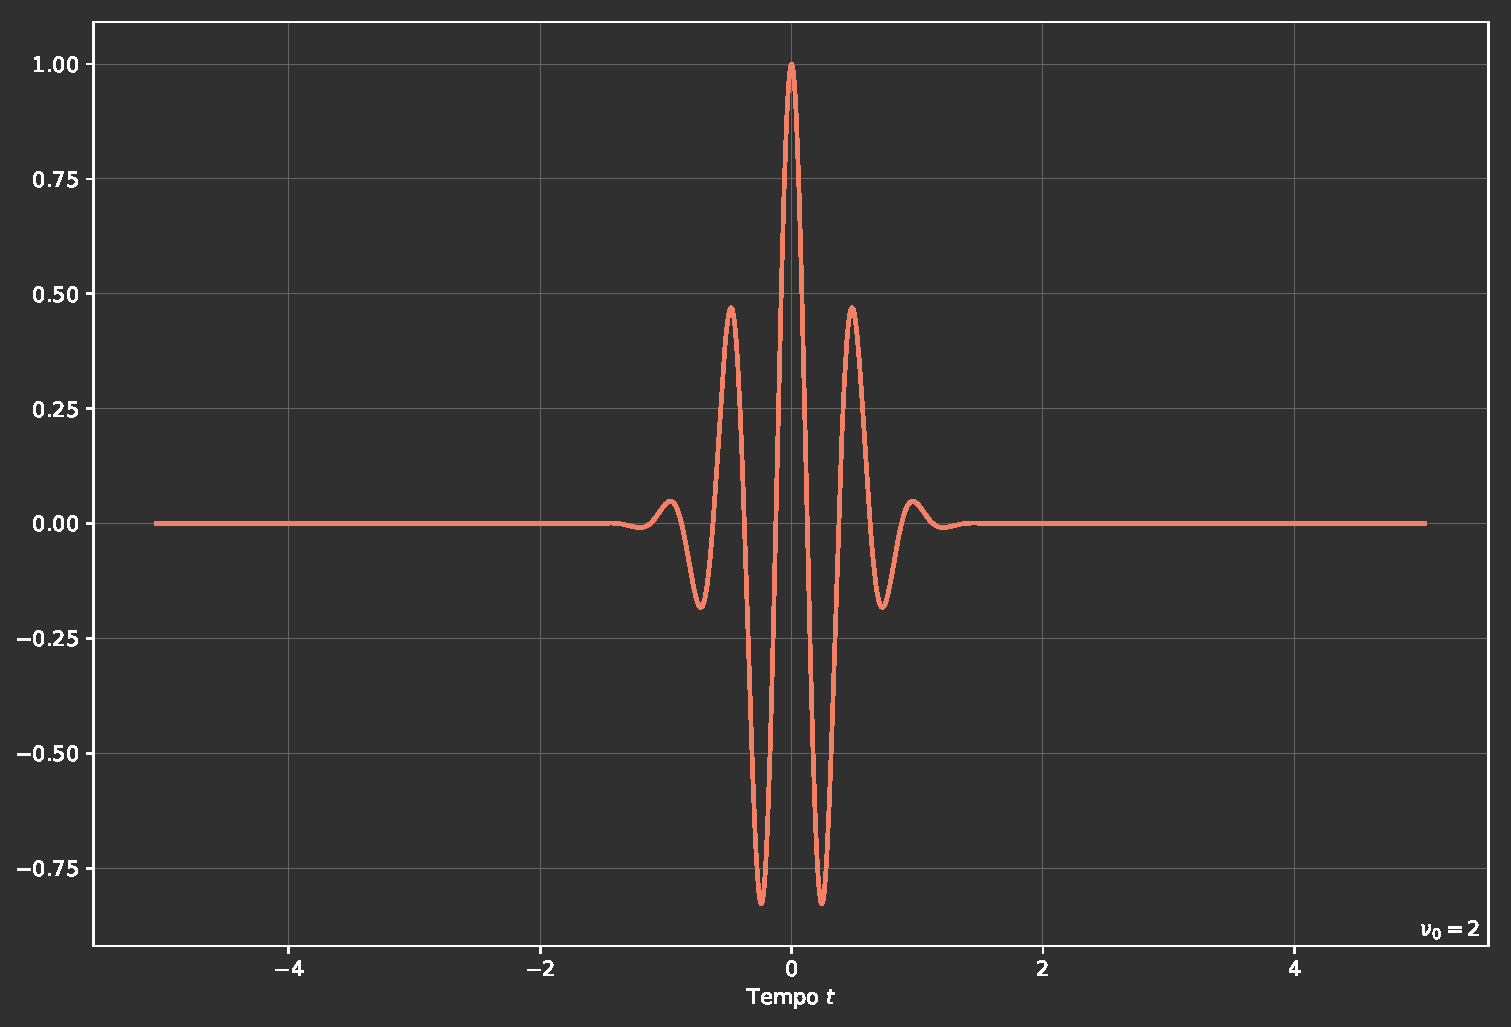
\includegraphics[height = 0.7 \textheight]{images/Pulse1.pdf}
    \end{frame}
    
    \begin{frame}{Fourier Transforming}
        \begin{equation*}
            \widehat{f}(\nu) = \frac{e^{-\pi(\nu - \nu_0)^2} + e^{-\pi(\nu + \nu_0)^2}}{2\sqrt{2\pi}}
        \end{equation*}
        \centering
        
        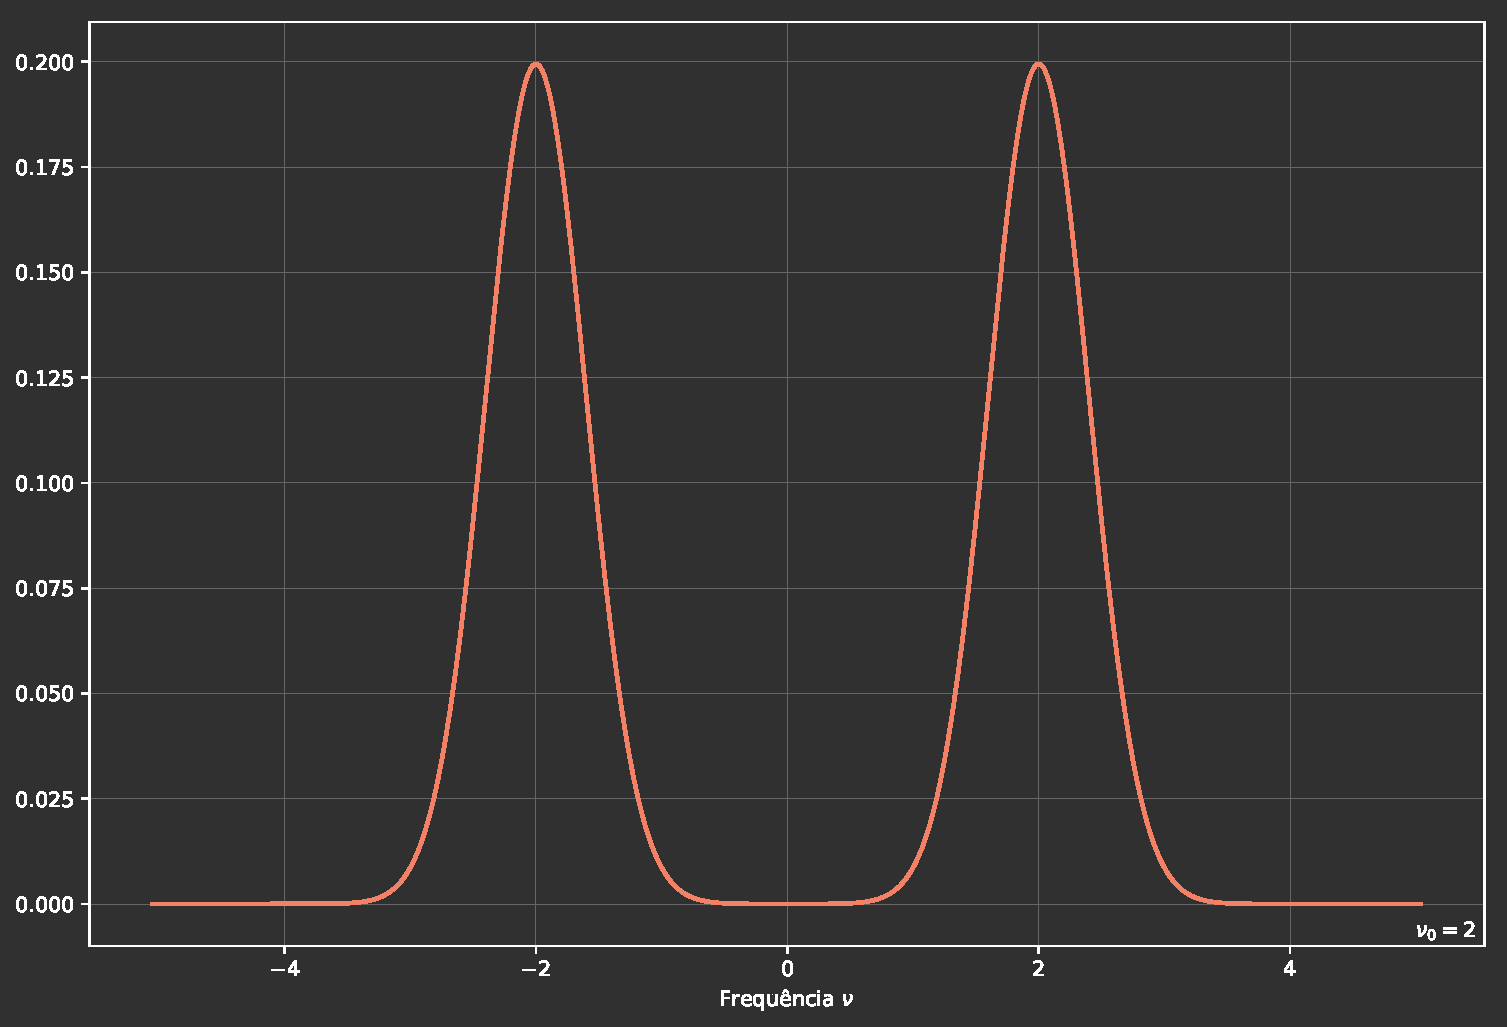
\includegraphics[height = 0.65 \textheight]{images/Pulse1-Fourier.pdf}
    \end{frame}
    
    \begin{frame}{A Harder Example}
        \uncover<+->{\begin{equation*}
            f(t) = e^{i\omega_0 t} = \cos(\omega_0 t) + i \sin(\omega_0 t)
        \end{equation*}}
        \uncover<+->{\begin{equation*}
            \widehat{f}(\omega) = \frac{1}{\sqrt{2\pi}} \int_{-\infty}^{+\infty} e^{i\omega_0 t} e^{-i \omega t} \dd{t}
        \end{equation*}}
    \end{frame}
    
    \begin{frame}{The Mathematical Moonwalk}
        \uncover<+->{\begin{equation*}
            f(t) = e^{i\omega_0 t}
        \end{equation*}}
        \uncover<+->{\begin{equation*}
            e^{i\omega_0 t} = \frac{1}{\sqrt{2\pi}} \int_{-\infty}^{+\infty} \widehat{f}(\omega) e^{i \omega t} \dd{\omega}
        \end{equation*}}
        \uncover<+->{\begin{equation*}
            \widehat{f}(\omega) = \sqrt{2\pi} \dirac{\omega - \omega_0}
        \end{equation*}}
    \end{frame}
    
    \begin{frame}{Cosines}
        \begin{equation*}
            f(t) = \cos(\omega_0 t) = \frac{e^{i\omega_0t} + e^{-i\omega_0t}}{2}
        \end{equation*}
        
        \centering
        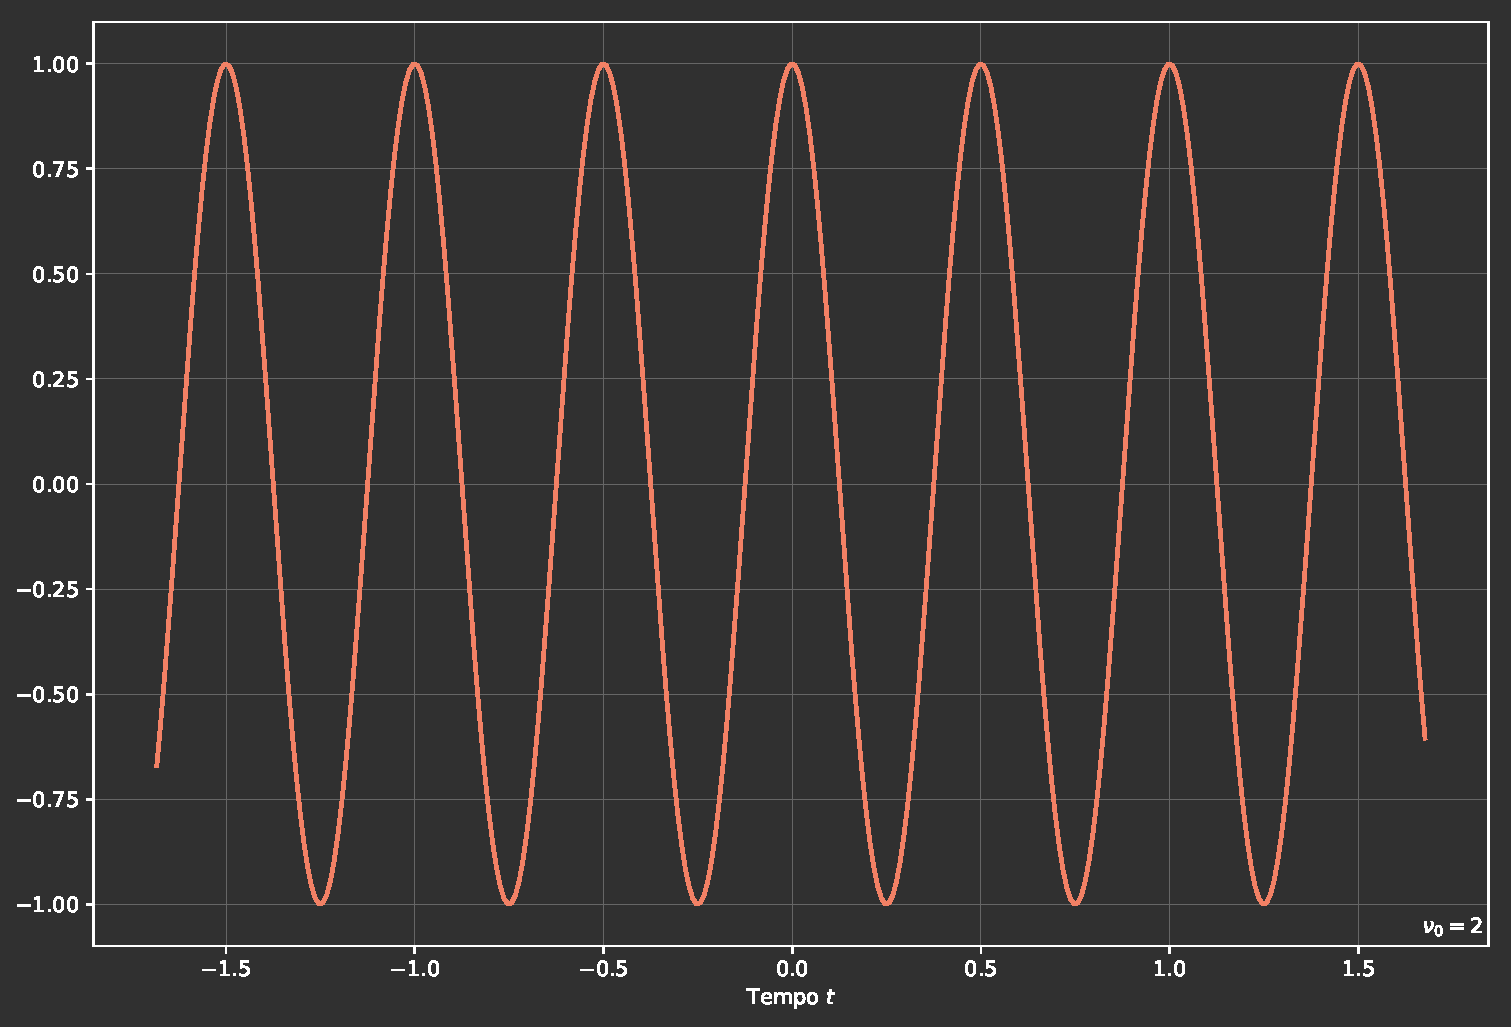
\includegraphics[height = 0.65 \textheight]{images/Pulse2.pdf}
    \end{frame}
    
    \begin{frame}{Cosines}
        \begin{equation*}
            \widehat{f}(\omega) = \sqrt{\frac{\pi}{2}}\prnt{\dirac{\omega-\omega_0} + \dirac{\omega+\omega_0}}    
        \end{equation*}
        
        \centering 
        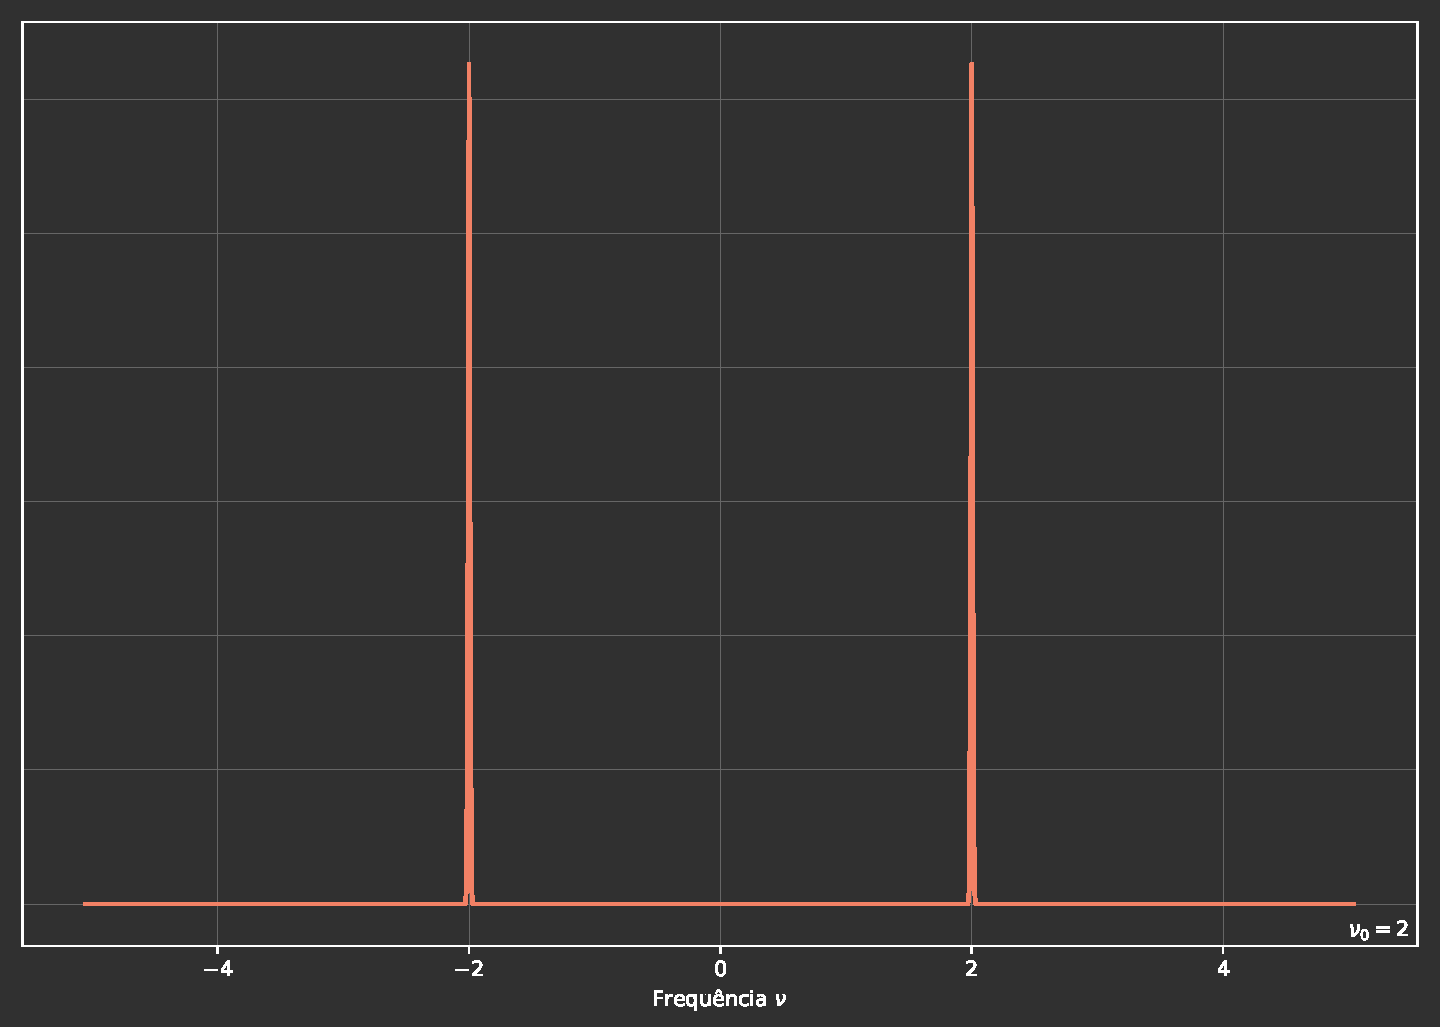
\includegraphics[height = 0.65 \textheight]{images/Pulse2-Fourier.pdf}
    \end{frame}